% généré depuis source/06_evaluation_visualisation.md — ne pas modifier à la main
\chapter{Évaluation et visualisation}\label{sec:evaluation}

\chapintro

Ce chapitre évalue d'abord la solution : protocole et métriques, puis résultats de fiabilité, de disponibilité, de détection de l'état critique et de RUL, et comparaison des méthodes. Il montre ensuite comment ces résultats sont restitués dans le tableau de bord et comment leur reproductibilité est assurée.

\section{Protocole et métriques}\label{sec:protocole}

Le découpage officiel de FD001 est respecté : les modèles sont appris sur les 100 moteurs d'entraînement et évalués sur les 100 moteurs de test. La fiabilité porte sur les 200 unités avec censure ; la classification est validée par GroupKFold puis évaluée sur tous les cycles de test ; la RUL est évaluée au dernier cycle observé de chaque moteur, comme dans le challenge PHM \cite{saxena2008damage}.

Pour la classification, la classe positive est l'état critique. Le \textbf{rappel} est la métrique prioritaire, car une défaillance manquée coûte bien plus qu'une inspection inutile ; l'AUC \cite{hanley1982} mesure la qualité du classement indépendamment du seuil. Pour la RUL, l'erreur d'un moteur est $e_i = \widehat{\mathrm{RUL}}_i - \mathrm{RUL}_i$ ; une erreur positive est une prédiction \textbf{tardive}, la plus dangereuse. Sur $N$ moteurs :

\begin{equation}\label{eq:rmse}
\mathrm{RMSE} = \sqrt{\frac1N \sum_i e_i^2}, \qquad \mathrm{MAE} = \frac1N \sum_i |e_i|, \qquad S = \sum_i \begin{cases} e^{-e_i/13} - 1 & e_i < 0 \\ e^{e_i/10} - 1 & e_i \ge 0 \end{cases},
\end{equation}

où $S$ est le score NASA \cite{saxena2008damage}. La \textbf{couverture} d'un intervalle de prédiction est la proportion de moteurs dont la RUL réelle y tombe ; elle doit être proche du niveau nominal.

\section{Fiabilité}\label{sec:res-fiabilite}

La figure~\ref{fig:fiabilite_kaplan_meier} compare l'estimateur KM aux lois ajustées ; la médiane de survie vaut 202 cycles. Les censures, concentrées aux faibles âges, élargissent peu l'IC. Le taux de Nelson-Aalen, nul avant la première défaillance puis croissant, confirme une \textbf{usure}.

\begin{figure}[htbp]
\centering
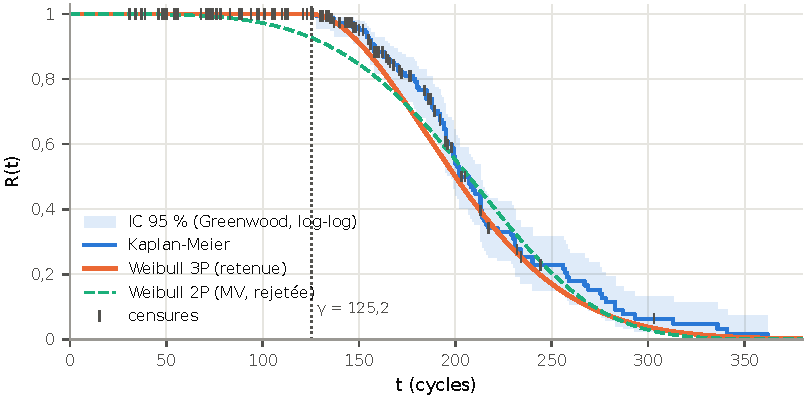
\includegraphics[width=1\linewidth]{figures/fiabilite_kaplan_meier.pdf}
\caption{Fonction de fiabilité : estimateur KM avec son IC et les censures, loi de Weibull 3P retenue et loi de Weibull 2P (MV) rejetée.}\label{fig:fiabilite_kaplan_meier}
\end{figure}

Le diagramme de Weibull (figure~\ref{fig:fiabilite_diagramme_weibull}) est nettement courbé ($R^2 = 0{,}894$, $\beta = 5{,}52$ par MCO), ce qui révèle un paramètre de position non nul.

\begin{figure}[htbp]
\centering
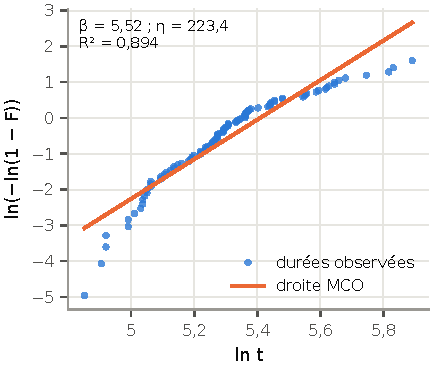
\includegraphics[width=0.55\linewidth]{figures/fiabilite_diagramme_weibull.pdf}
\caption{Diagramme de Weibull (rangs de Bernard) et droite des MCO : la courbure révèle un paramètre de position non nul.}\label{fig:fiabilite_diagramme_weibull}
\end{figure}

Le tableau~\ref{tab:fiabilite_adequation} compare les quatre lois candidates.

\begin{table}[htbp]
\centering\small
\begin{adjustbox}{max width=\linewidth,center}
\begin{tabular}{lrrrrrl}
\toprule
Loi & Paramètres & Log-vraisemblance & AIC & KS D & KS p & Décision (\ensuremath{\alpha} = 5 \%) \\
\midrule
Exponentielle & 1 & \ensuremath{-}632,94 & 1\,267,88 & 0,470 & 0,000 & rejetée \\
Weibull 2P & 2 & \ensuremath{-}530,75 & 1\,065,50 & 0,157 & 0,013 & rejetée \\
Log-normale & 2 & \ensuremath{-}517,46 & 1\,038,91 & 0,094 & 0,317 & acceptée \\
Weibull 3P & 3 & \ensuremath{-}516,52 & 1\,039,03 & 0,094 & 0,319 & acceptée \\
\bottomrule
\end{tabular}
\end{adjustbox}
\caption{Adéquation des lois candidates (MV sur les durées complètes)}\label{tab:fiabilite_adequation}
\end{table}

La loi exponentielle et la Weibull 2P (MV, $\beta = 4{,}41$, $p = 0{,}013$) sont rejetées. La Weibull 3P et la log-normale sont acceptées et équivalentes ($\Delta\mathrm{AIC} = 0{,}12$). La \textbf{Weibull 3P est retenue} : $\gamma = 125{,}2$ cycles traduit une période sans défaillance cohérente avec la première défaillance à 128 cycles, $\beta = 1{,}83 > 1$ un taux croissant, et c'est la loi de référence du cours \cite{benhmida}. L'ajustement 2P avec censure donne une échelle plus grande ($\eta = 236{,}6$ cycles), car les moteurs censurés ont survécu au moins jusqu'à leur dernier cycle. Le tableau~\ref{tab:fiabilite_indicateurs} donne les indicateurs du modèle retenu.

\begin{table}[htbp]
\centering\small
\begin{adjustbox}{max width=\linewidth,center}
\begin{tabular}{lrl}
\toprule
Indicateur & Valeur & Source \\
\midrule
MTTF = \ensuremath{\gamma} + \ensuremath{\eta}·\ensuremath{\Gamma}(1 + 1/\ensuremath{\beta}) & 206,3 cycles & Weibull 3P \\
B1 (1 \% de défaillances) & 132,6 cycles & Weibull 3P \\
B10 (10 \%) & 151,9 cycles & Weibull 3P \\
B50 (médiane) & 199,9 cycles & Weibull 3P \\
Médiane de survie & 202 cycles & Kaplan-Meier \\
Aire sous la courbe de survie & 214,3 cycles & Kaplan-Meier \\
Première défaillance observée & 128 cycles & données \\
\bottomrule
\end{tabular}
\end{adjustbox}
\caption{Indicateurs de fiabilité}\label{tab:fiabilite_indicateurs}
\end{table}

$B_{50}$ est proche de la médiane KM, ce qui confirme l'accord des deux approches au centre de la distribution. La figure~\ref{fig:fiabilite_densite_repartition} situe $B_{10}$ et $B_{50}$ sur la densité et la fonction de répartition.

\begin{figure}[htbp]
\centering
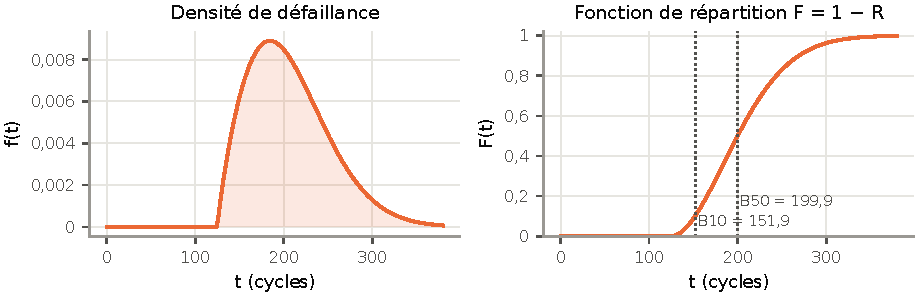
\includegraphics[width=1\linewidth]{figures/fiabilite_densite_repartition.pdf}
\caption{Densité de défaillance et fonction de répartition de la loi de Weibull 3P, avec les durées B10 et B50.}\label{fig:fiabilite_densite_repartition}
\end{figure}

\section{Disponibilité et remplacement préventif}\label{sec:res-fmds02}

Le tableau~\ref{tab:fmds_maintenabilite_disponibilite} regroupe les indicateurs obtenus avec les temps de réparation simulés.

\begin{table}[htbp]
\centering\small
\begin{adjustbox}{max width=\linewidth,center}
\begin{tabular}{ll}
\toprule
Grandeur & Valeur \\
\midrule
Loi des temps de réparation (MV) & log-normale, \ensuremath{\mu} = 2,742, \ensuremath{\sigma} = 0,464 (KS p = 0,61) \\
MTTR & 17,3 h = 8,6 cycles \\
t90 (90 \% des réparations terminées) & 28,1 h \\
MUT / MDT / MTBF & 206,3 / 8,64 / 215,0 cycles \\
Disponibilité intrinsèque A = MUT / (MUT + MDT) & 95,98 \% \\
Âge optimal de remplacement T* & 130,7 cycles, R(T*) = 0,994 \\
Coût par cycle : à T* / corrective seule & 0,0078 / 0,0242 (unités de Cp) \\
Gain du préventif & 67,7 \% \\
\bottomrule
\end{tabular}
\end{adjustbox}
\caption{Maintenabilité, disponibilité et remplacement préventif (temps de réparation simulés)}\label{tab:fmds_maintenabilite_disponibilite}
\end{table}

La loi log-normale ré-estimée est acceptée par le test KS ($p = 0{,}61$). La disponibilité intrinsèque atteint \textbf{95,98 \%}, soit environ 40,2 h d'indisponibilité pour mille heures. La figure~\ref{fig:fmds_remplacement_preventif} montre le coût du remplacement préventif en fonction de l'âge.

\begin{figure}[htbp]
\centering
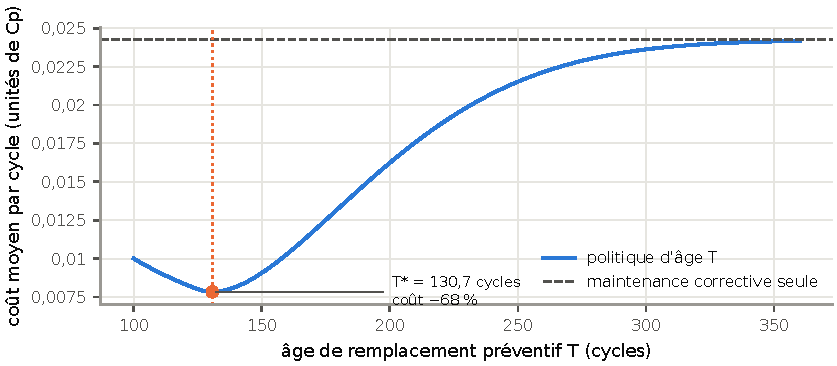
\includegraphics[width=1\linewidth]{figures/fmds_remplacement_preventif.pdf}
\caption{Coût moyen par cycle du remplacement à âge fixe en fonction de l'âge T, comparé à la maintenance corrective seule.}\label{fig:fmds_remplacement_preventif}
\end{figure}

L'optimum, net, se situe à $T^* = 130{,}7$ cycles, juste après la période sans défaillance : le coût par cycle baisse de \textbf{68 \%}, au prix d'un remplacement en moyenne 75,6 cycles avant le MTTF.

\section{Détection de l'état critique}\label{sec:res-sante}

Parmi les capteurs non constants, 12 dépassent le seuil de tendance et sont retenus : s2, s3, s4, s7, s8, s11, s12, s13, s15, s17, s20, s21. La figure~\ref{fig:sante_indicateur} montre le HI obtenu.

\begin{figure}[htbp]
\centering
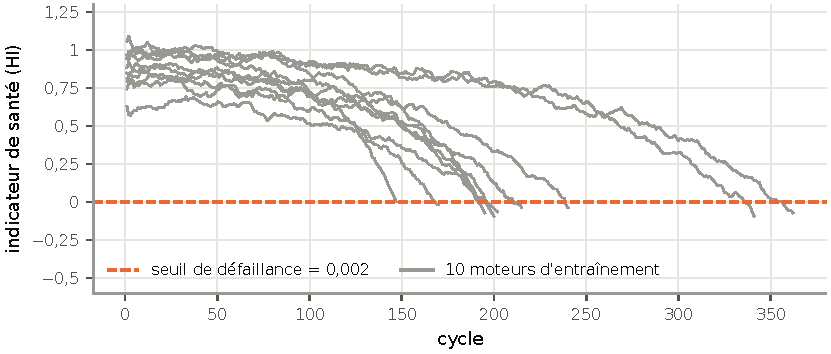
\includegraphics[width=1\linewidth]{figures/sante_indicateur.pdf}
\caption{HI lissé de dix moteurs d'entraînement et seuil de défaillance.}\label{fig:sante_indicateur}
\end{figure}

Le HI part d'environ un et décroît jusqu'au voisinage de zéro pour tous les moteurs, quelle que soit leur durée de vie. Le tableau~\ref{tab:sante_classifieurs} compare les deux classifieurs.

\begin{table}[htbp]
\centering\small
\begin{adjustbox}{max width=\linewidth,center}
\begin{tabular}{llrrrrr}
\toprule
Modèle & Évaluation & AUC & Exactitude & Précision & Rappel & F1 \\
\midrule
Gradient Boosting & validation croisée (GroupKFold 5) & 0,990 & 0,961 & 0,892 & 0,844 & 0,867 \\
 & test NASA & 0,991 & 0,986 & 0,747 & 0,657 & 0,699 \\
SVM (RBF) & validation croisée (GroupKFold 5) & 0,983 & 0,958 & 0,879 & 0,824 & 0,851 \\
 & test NASA & 0,974 & 0,986 & 0,798 & 0,621 & 0,698 \\
\bottomrule
\end{tabular}
\end{adjustbox}
\caption{Classification normal / critique (RUL \ensuremath{\le} 30 cycles)}\label{tab:sante_classifieurs}
\end{table}

Les deux modèles séparent très bien les classes ; le \textbf{gradient boosting}, de meilleure AUC sur le test (0,991), est retenu. Son rappel de test (0,657) est pourtant inférieur à celui de la validation croisée (0,844), comme le détaille la figure~\ref{fig:sante_matrice_confusion}.

\begin{figure}[htbp]
\centering
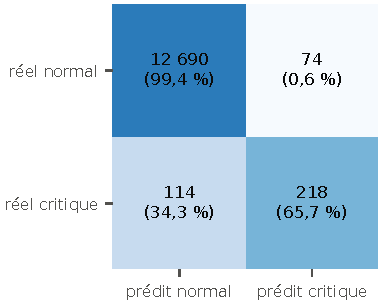
\includegraphics[width=0.50\linewidth]{figures/sante_matrice_confusion.pdf}
\caption{Matrice de confusion du gradient boosting sur le jeu de test, au seuil de décision par défaut.}\label{fig:sante_matrice_confusion}
\end{figure}

Le jeu de test est très déséquilibré : la plupart des séries s'arrêtent bien avant la défaillance. L'AUC reste élevée, c'est donc le seuil de décision qui est trop strict. Au dernier cycle, la flotte compte 76 moteurs normaux, 4 en surveillance et 20 critiques.

\section{Durée de vie résiduelle}\label{sec:res-rul}

Le tableau~\ref{tab:rul_metriques} compare les deux modèles sur les 100 moteurs de test.

\begin{table}[htbp]
\centering\small
\begin{adjustbox}{max width=\linewidth,center}
\begin{tabular}{lrrrrrr}
\toprule
Modèle & RMSE & MAE & Biais & Score NASA & |e| \ensuremath{\le} 15 & Tardives \\
\midrule
Dégradation bayésienne & 24,47 & 18,98 & +13,5 & 3\,743 & 49 \% & 78 \% \\
LSTM & 15,35 & 11,22 & +2,2 & 485 & 68 \% & 58 \% \\
Moyenne des deux & 16,91 & 13,49 & +7,9 & 600 & 64 \% & 76 \% \\
\bottomrule
\end{tabular}
\end{adjustbox}
\caption{Performances des modèles de RUL sur les 100 moteurs de test}\label{tab:rul_metriques}
\end{table}

Le \textbf{LSTM est le plus précis} sur toutes les métriques et presque sans biais. Le modèle de dégradation prédit en moyenne trop tard (+13,5 cycles), ce que le score NASA amplifie. La moyenne des deux n'améliore pas le LSTM seul. La figure~\ref{fig:rul_predit_vs_reel} montre les prédictions en fonction de la RUL réelle.

\begin{figure}[htbp]
\centering
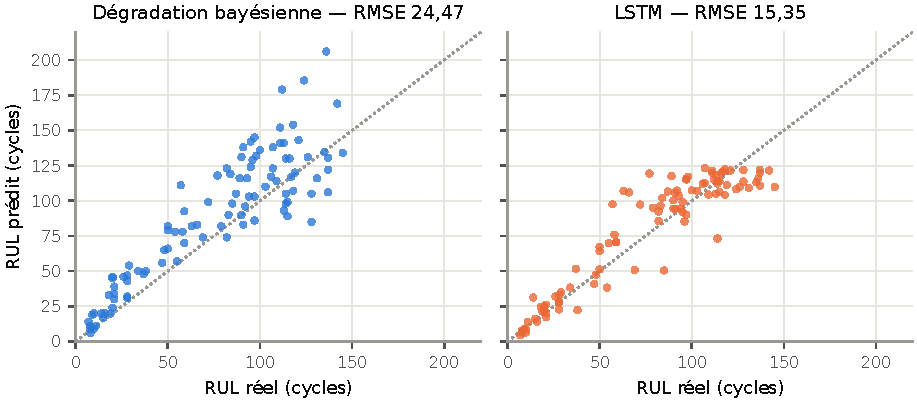
\includegraphics[width=1\linewidth]{figures/rul_predit_vs_reel.pdf}
\caption{RUL prédite en fonction de la RUL réelle pour les deux modèles ; la diagonale correspond à une prédiction parfaite.}\label{fig:rul_predit_vs_reel}
\end{figure}

Le LSTM suit la diagonale jusqu'à son plafond de 125 cycles ; le modèle de dégradation est plus dispersé et majoritairement au-dessus. La figure~\ref{fig:rul_calibration} évalue ses intervalles de prédiction.

\begin{figure}[htbp]
\centering
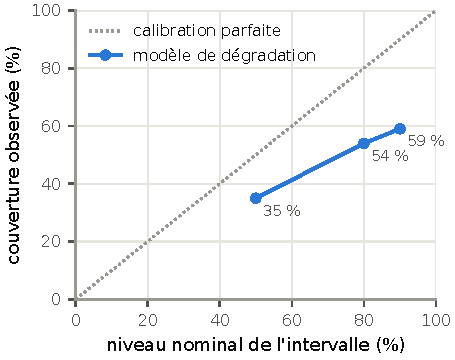
\includegraphics[width=0.55\linewidth]{figures/rul_calibration.pdf}
\caption{Calibration des intervalles du modèle de dégradation : couverture observée en fonction du niveau nominal.}\label{fig:rul_calibration}
\end{figure}

Les couvertures observées, 35 \%, 54 \% et 59 \% pour des niveaux nominaux de 50, 80 et 90 \%, sont toutes trop faibles : \textbf{les intervalles sont trop étroits} et le modèle sous-estime son incertitude. La figure~\ref{fig:rul_exemple_moteur} illustre les deux modèles sur le moteur de test n° 31.

\begin{figure}[htbp]
\centering
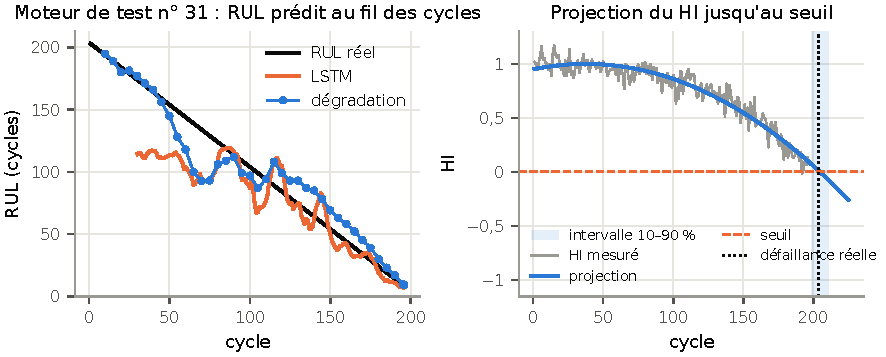
\includegraphics[width=1\linewidth]{figures/rul_exemple_moteur.pdf}
\caption{Moteur de test pris en exemple : RUL prédite à chaque cycle par les deux modèles (gauche) et projection du HI jusqu'au seuil de défaillance (droite).}\label{fig:rul_exemple_moteur}
\end{figure}

Au fil des cycles, les deux prédictions se rapprochent de la RUL réelle (8 cycles) ; la projection du HI montre comment le modèle bayésien déduit la RUL du franchissement du seuil.

\section{Comparaison des méthodes}\label{sec:comparaison}

Les deux approches de RUL sont complémentaires. Le \textbf{LSTM} est précis et quasi sans biais, du même ordre que les réseaux récurrents publiés sur FD001 \cite{zheng2017,ramasso2014}, mais il ne fournit pas d'incertitude et reste peu interprétable. Le \textbf{modèle de dégradation} est moins précis et biaisé, mais chaque étape est interprétable et il fournit une distribution de la RUL, encore mal calibrée. En fiabilité, les approches non paramétrique et paramétrique concordent sur la forme du taux et sur la médiane.

\section{Visualisation : le tableau de bord}\label{sec:dashboard}

Les résultats évalués sont restitués dans un tableau de bord web React, alimenté par une API qui sert les fichiers de résultats ; une version autonome en un seul fichier HTML s'ouvre sans serveur. La page de vue d'ensemble (figure~\ref{fig:dashboard_overview}) réunit les indicateurs clés et l'état de la flotte.

\begin{figure}[htbp]
\centering
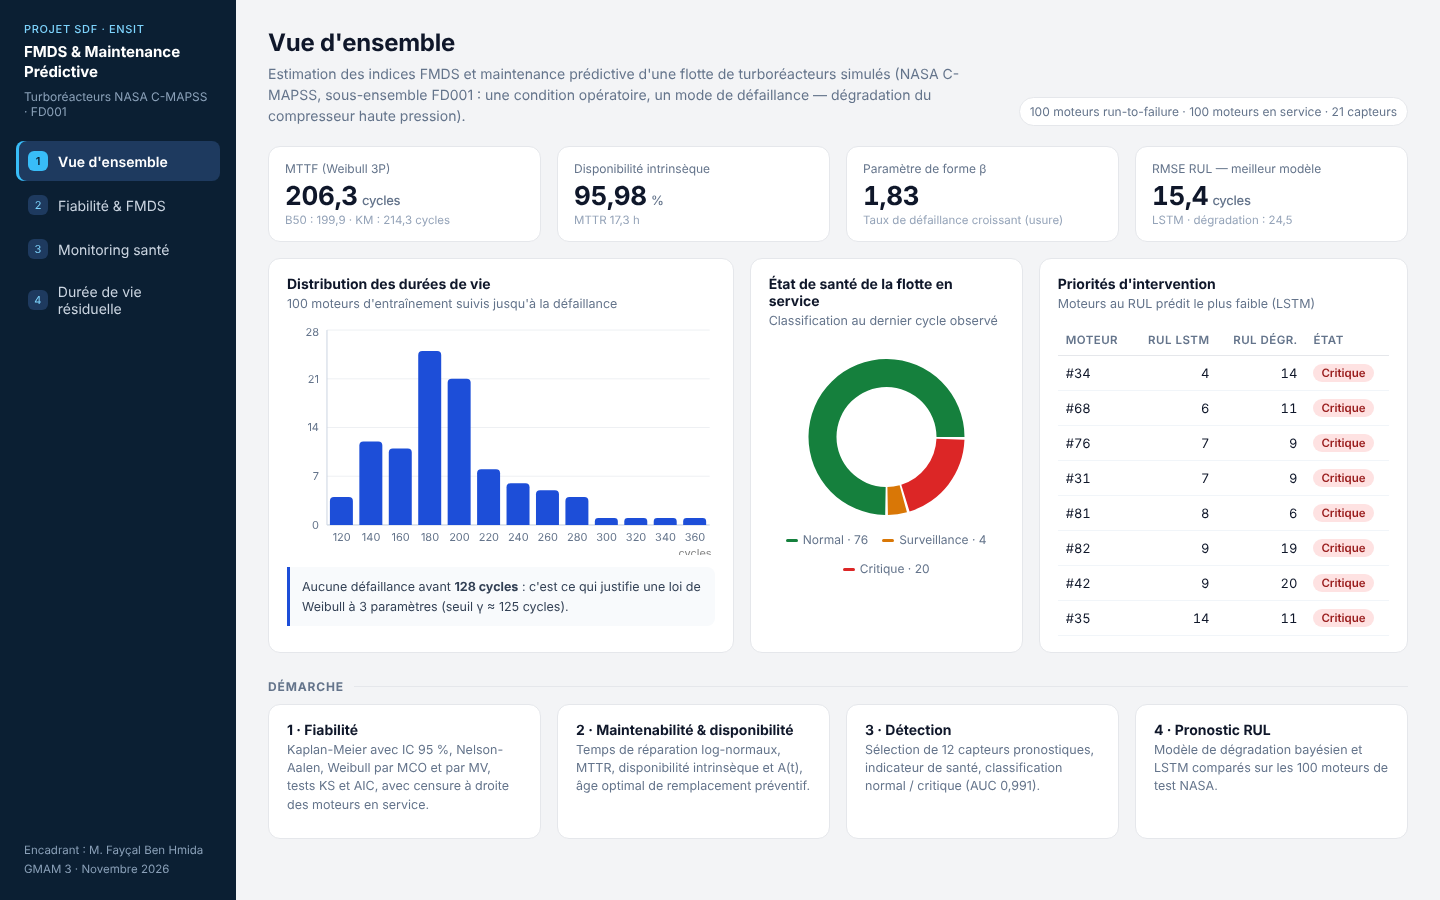
\includegraphics[width=1\linewidth]{figures/dashboard_overview.png}
\caption{Page de vue d'ensemble : indicateurs clés, distribution des durées de vie, état de la flotte et priorités d'intervention.}\label{fig:dashboard_overview}
\end{figure}

La page consacrée à la RUL (figure~\ref{fig:dashboard_rul}) compare les deux modèles et détaille les prédictions pour chaque moteur.

\begin{figure}[htbp]
\centering
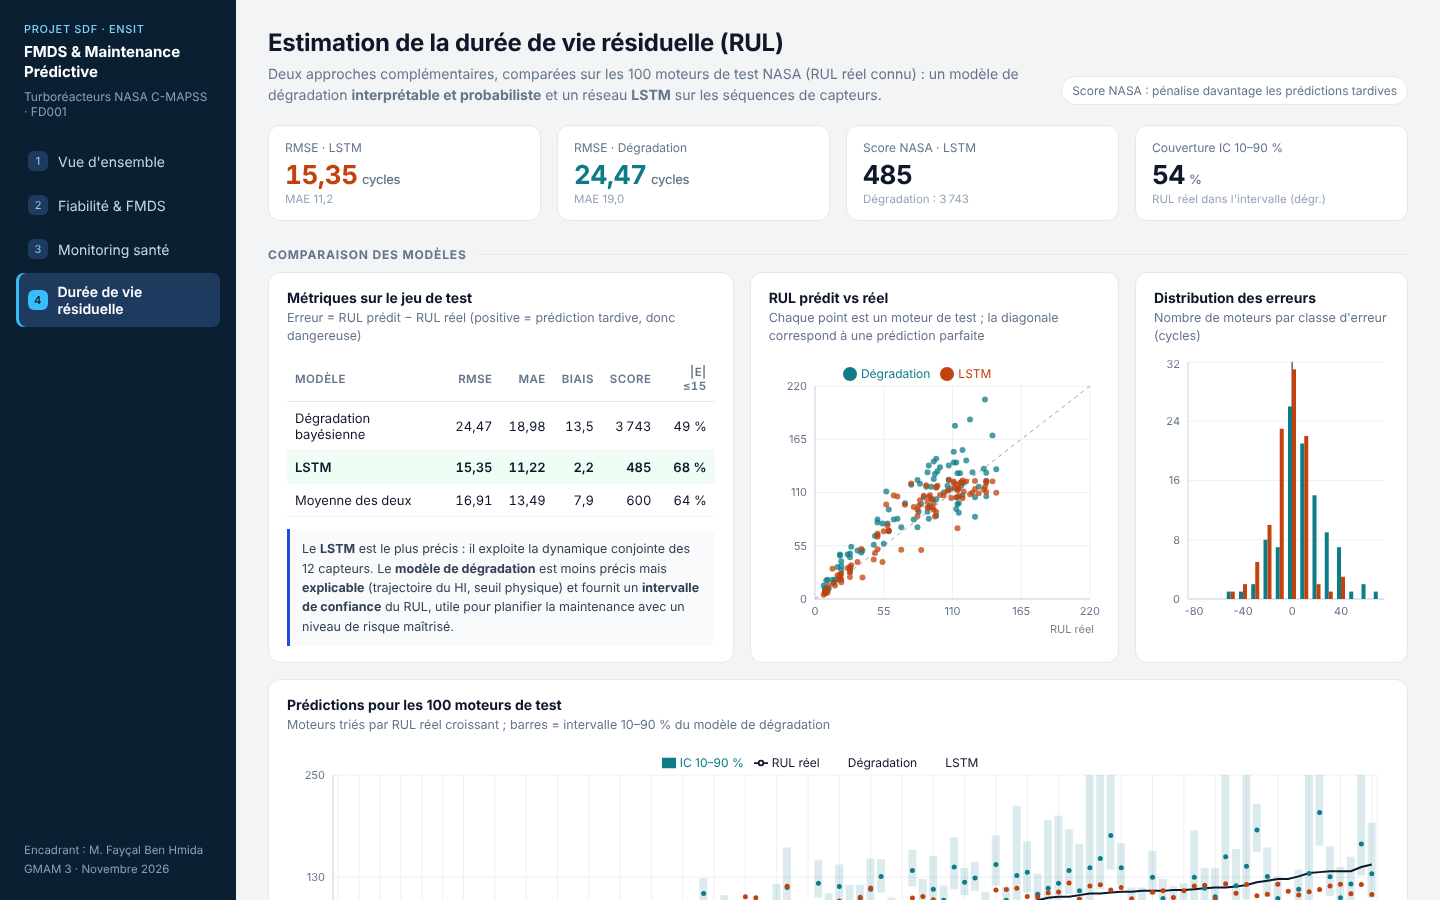
\includegraphics[width=1\linewidth]{figures/dashboard_rul.png}
\caption{Page de la durée de vie résiduelle : métriques des deux modèles, prédictions et erreurs.}\label{fig:dashboard_rul}
\end{figure}

\section{Reproductibilité}\label{sec:reproductibilite}

Toutes les étapes aléatoires utilisent des graines fixées, et chaque exécution enregistre les versions des bibliothèques (Python 3.12.10, scikit-learn 1.9.1, PyTorch 2.15.0). Le réentraînement du LSTM variant légèrement d'une machine à l'autre, les résultats publiés correspondent au modèle sauvegardé. Une suite de tests automatiques vérifie les méthodes, l'absence de fuite entre moteurs et la concordance de chaque nombre du rapport avec sa source.

\chapconclusion

La Weibull 3P décrit la fiabilité de la flotte avec un MTTF de 206,3 cycles, le classifieur atteint une AUC de 0,991, et le LSTM est le plus précis pour la RUL (RMSE de 15,35 cycles), tandis que le modèle de dégradation fournit des intervalles encore trop étroits. Le chapitre suivant discute ces résultats.
